%!TeX program = xelatex
%Do not change
\documentclass[12pt, oneside]{article}
\usepackage{amssymb,amsmath}
\usepackage[margin=1in]{geometry}
\usepackage{textpos}
\usepackage{float}
\usepackage{booktabs}
%\usepackage{color}
\usepackage{graphicx}
\usepackage[inter-unit-product =\cdot]{siunitx}
\let\DeclareUSUnit\DeclareSIUnit
\let\US\SI
\DeclareUSUnit\inch{in}
\DeclareUSUnit\foot{ft}
\DeclareUSUnit\mile{mi}
\DeclareUSUnit\foot{ft}
\DeclareUSUnit\slug{slug}
\DeclareUSUnit\pound{lb}
\DeclareUSUnit\psi{psi}
\DeclareUSUnit\Msi{Msi}
\DeclareUSUnit\ksi{ksi}

\usepackage{tikz}
\usetikzlibrary{positioning}
%\usepackage{tikz-3dplot}
\usepackage{pgfopts}
%\usepackage{wasysym}
\usepackage{stanli}

% You may add the packages you need here
\begin{document}

%TODO change numbers in problems
\begin{textblock*}{4cm}(-1.7cm,-2.3cm)
\noindent {\scriptsize AE333 Fall 2021}
\end{textblock*}

%Do not modify other than putting your name where stated
\begin{textblock*}{8cm}(12.5cm,-1cm)
\noindent {Name: }
\end{textblock*}
%Do not modify other than typing your acknowledgement where stated
\begin{textblock*}{13.5cm}(-1.7cm,-1.8cm)
%\noindent \textit{\footnotesize Acknowledgement: Your acknowledgement for collaboration and other sources goes here. }
\end{textblock*}

\vspace{1cm}

%Do not modify other than typing the homework number after #
\begin{center}
\textbf{\Large Homework 10 Solutions}

\textbf{Not for credit}
\end{center}

\begin{enumerate}
	\item %12-99
		Find the reactions at each support, assume $EI$ is constant and neglect axial load.
		\begin{figure}[H]
			\centering
			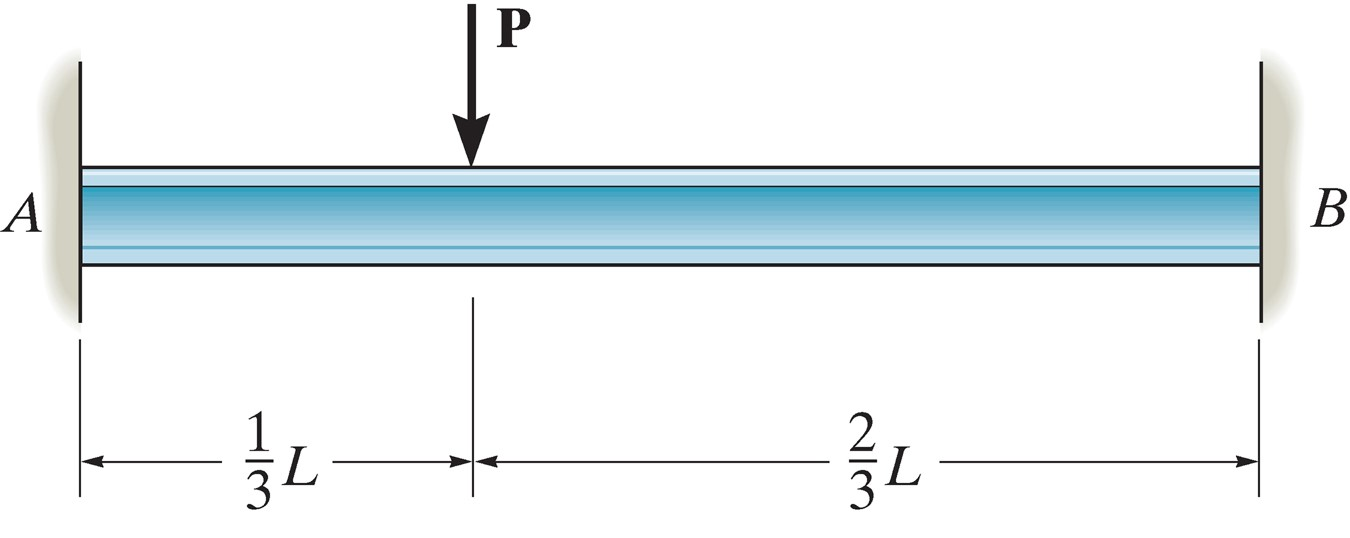
\includegraphics[width=0.6\linewidth]{12-99}
		\end{figure}
			\textbf{Solution:}
			\begin{itemize}
				\item With a beam fixed at both ends we can find from statics that $A + B = P$ and from the sum of moments about $A$ we find $M_B + BL = PL/3$.
				\item We have boundary conditions of $v(0) = v(L) = dv/dx(0) = dv/dx(L) = 0$.
				\item Because the internal moment equation for this problem is discontinuous (we would have one moment function before the load $P$ and another after it) I will instead use discontinuity functions.
				\item $M(x) = Ax + M_A - P \langle x-L/3 \rangle$
				\item Integrating twice gives
					\begin{align*}
						EI \frac{dv}{dx} &= \frac{1}{2} Ax^2 + M_A x - \frac{P}{2} \langle x-L/3 \rangle^2 + C_1\\
						EI v &= \frac{1}{6} Ax^3 + \frac{1}{2} M_A x^2 - \frac{P}{6} \langle x-L/3 \rangle^3 + C_1x + C_2
					\end{align*}
				\item Applying the boundary conditions at $x=0$ gives $C_1 = C_2 = 0$.
				\item Applying the boundary conditions at $x=L$ gives $M_A = -\frac{4}{27}PL$ and $A = \frac{20}{27}P$
				\item Substituting into our original statics expressions gives $B = \frac{7}{27}P$ and $M_B = \frac{2PL}{27}$
			\end{itemize}

	\item %12-106
		Find the maximum deflection in terms of some constant $EI$
		\begin{figure}[H]
			\centering
			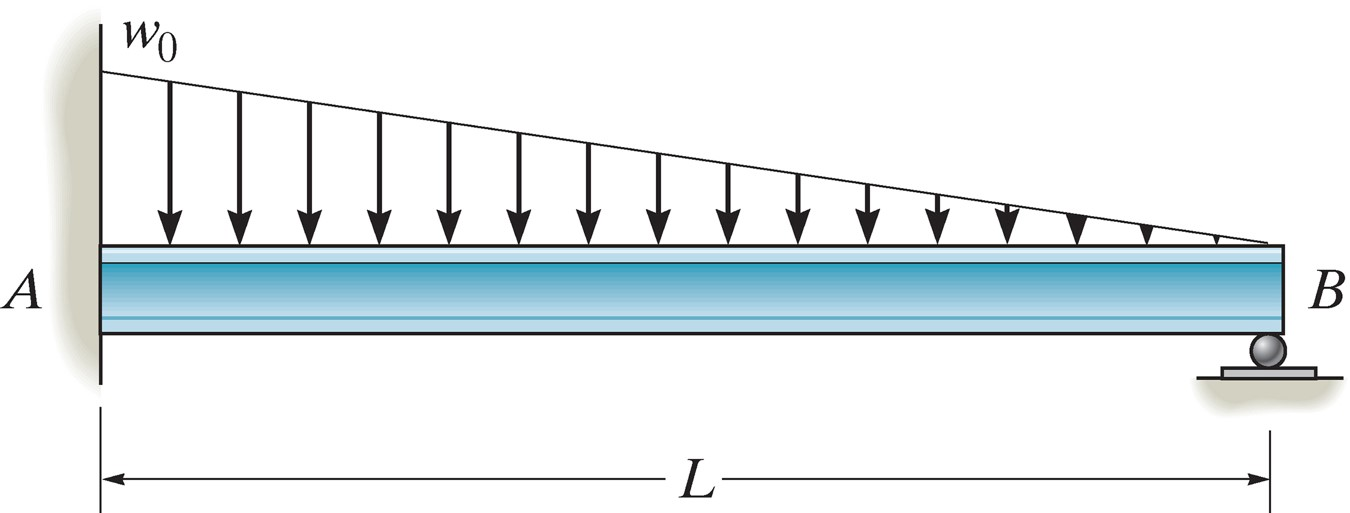
\includegraphics[width=0.6\linewidth]{12-106}
		\end{figure}
			\textbf{Solution:}
			\begin{itemize}
				\item For this problem it is convenient to use the superposition method
				\item We can add a cantilever beam with a distributed load as shown in the problem to a cantilever with an end load
				\item We need to choose an end-load such that the end deflections cancel, using the maximum deflections given in appendix C we find $\frac{w_0 L^4}{30 EI} = \frac{PL^3}{3EI}$
				\item And we find $P = \frac{w_0 L}{10}$
				\item To find the maximum deflection we need to add the two expressions for deflection and find when their derivative is equal to zero. Since these are higher order polynomials, it is best to do this using either a graphing calculator or some other software
				\item There are 4 roots to the equation, however only one is within our bounds ($x \approx 0.553 L$) which gives $v_max = -0.0239 \frac{w_0L^4}{EI}$
			\end{itemize}

	\item %12-107
		Find the maximum deflection in terms of some constant $EI$
		\begin{figure}[H]
			\centering
			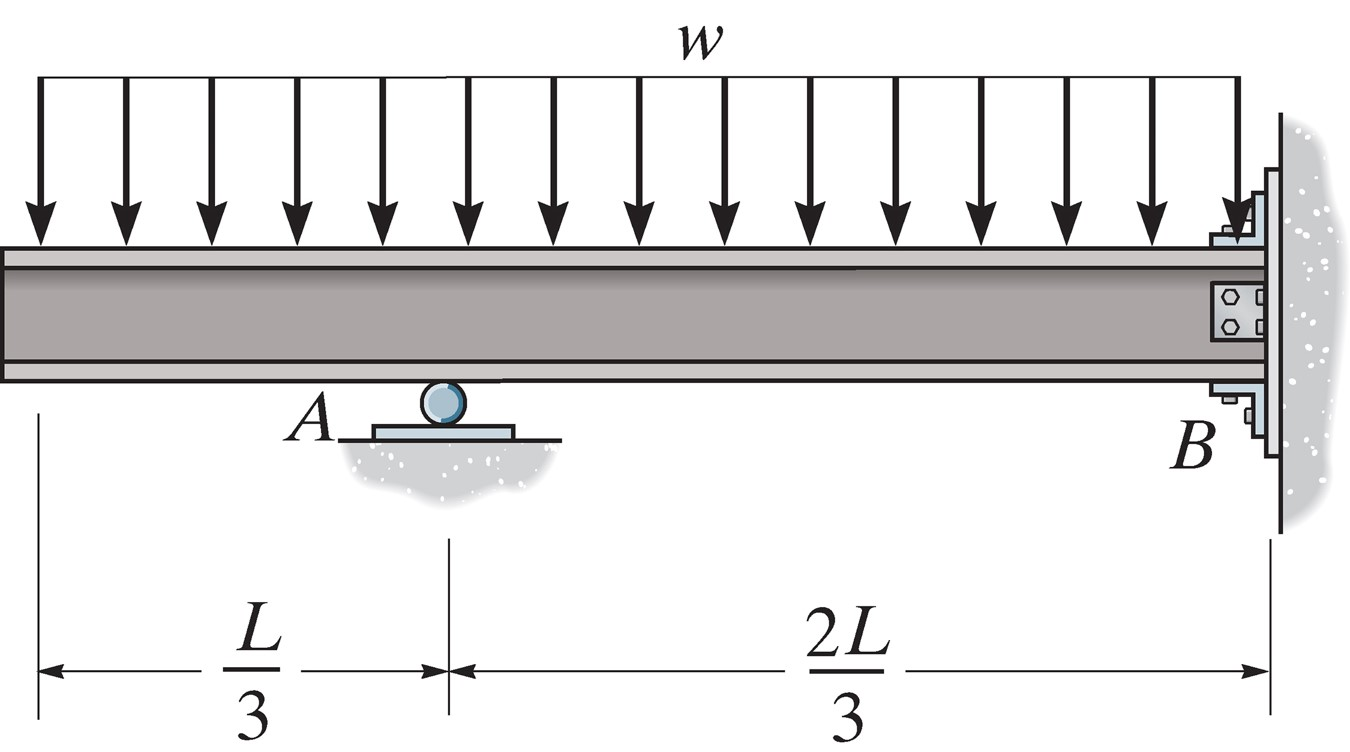
\includegraphics[width=0.6\linewidth]{12-107}
		\end{figure}
			\textbf{Solution:}
			\begin{itemize}
				\item For this problem I will once again use direct integration with discontinuity functions.
				\item From statics we know that $A + B = wL$ and that $M_B = \frac{2AL}{3} - \frac{wL^2}{2}$
				\item Setting our origin at the left we have boundary conditions of $v(L/3) = v(L) = dv/dx(L) = 0$. NOTE: This problem would be much easier to work by hand setting the origin on the right hand side and moving left, but either case should give the same answer, if you did that just substitute $x_{new} = L - x_{old}$
				\item Our moment function is $M = -w/2 x^2 + A\langle x - L/3 \rangle$
				\item And integrating twice yields
					\begin{align*}
						EI \frac{dv}{dx} &= -\frac{wx^3}{6} + \frac{A}{2} \langle x - L/3 \rangle^2 + C_1\\
						EI v &= -\frac{wx^4}{24} + \frac{A}{6} \langle x - L/3 \rangle^3 + C_1x + C_2
					\end{align*}
				\item We find that $A = \frac{17wL}{24}$, $B = \frac{7 wL}{24}$, $M_B = -\frac{wL^2}{36}$, $C_1 = \frac{wL^3}{108}$ and $C_2 = -\frac{5wL^4}{1944}$
				\item Using the same method as before, solving for $dv/dx=0$ we find possible locations for the maximum deflection at $x=0L, 0.405L, 0.720L$ so we compare the deflection at each location and find the maximum is at $x=0$ and is $v(0) = \frac{-5wL^4}{1944EI}$
			\end{itemize}

	\item %12-121
		Find the reactions at each of the supports, assuming $A$ is a fixed support and $B$ is a roller.
		\begin{figure}[H]
			\centering
			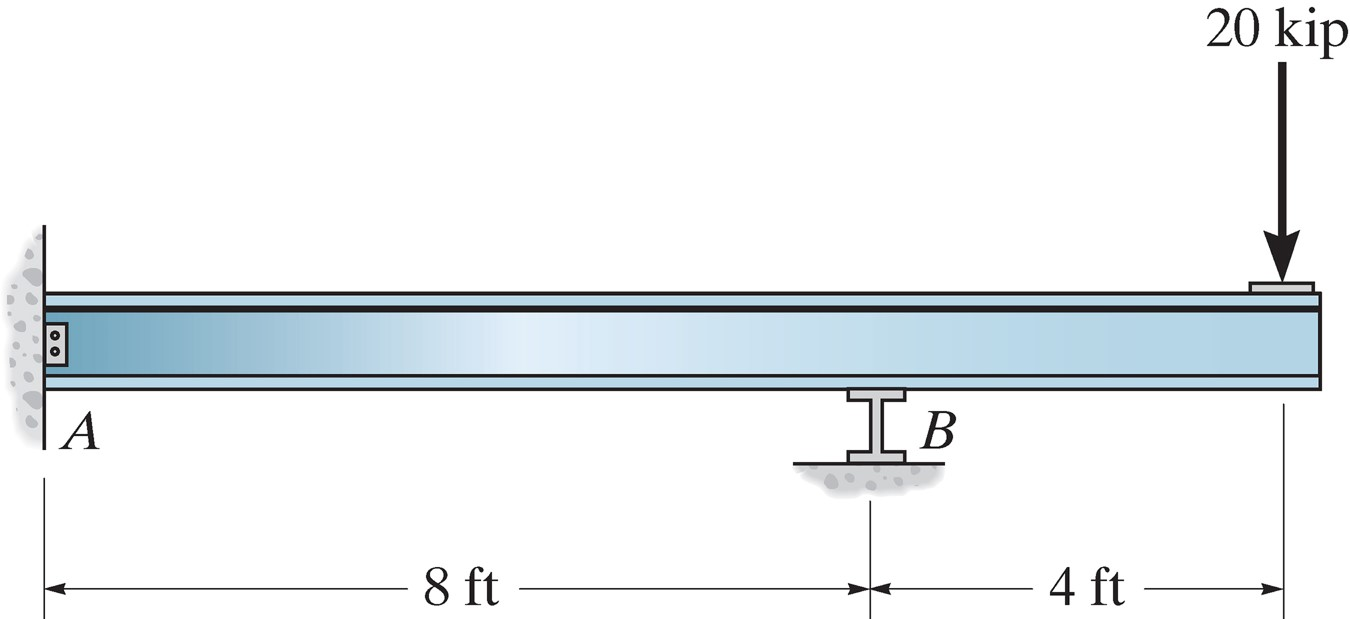
\includegraphics[width=0.6\linewidth]{12-121}
		\end{figure}
			\textbf{Solution:}
			\begin{itemize}
				\item Although this problem is simplest using discontinuity functions, I will demonstrate using direct integration without discontinuity functions for this solution
				\item We know from statics that $A+B = 20$ and that $M_A = 8B - 240$
				\item We find the following moment equations
					\begin{align*}
						M_1(x) &= Ax + M_A\\
						M_2(x) &= Ax + M_A + B(x-8)
					\end{align*}
				\item Integrating twice gives
					\begin{align*}
						EI dv_1/dx &= \frac{1}{2}Ax^2 + M_A x + C_1\\
						Ei v_1 &= \frac{1}{6}Ax^3 + \frac{1}{2} M_A x^2 + C_1 x + C_2\\
						EI dv_2/dx &=  \frac{1}{2}Ax^2 + M_A x + \frac{B}{2}(x-8)^2 + C_3\\
						EI v_2 &=  \frac{1}{6}Ax^3 + \frac{1}{2} M_A x^2 + \frac{B}{6}(x-8)^3 + C_3x + C_4
					\end{align*}
				\item We have 7 unknowns with 2 statics equations, 3 boundary conditions ($v(0) = dv/dx(0) = v(8) = 0$) and 2 continuity equations ($v_1(8) = v_2(8)$, $dv_1/dx(8) = dv_2/dx(8)$), which in total makes 7 equations, so we should be able to solve for all the unknowns.
				\item It is quick to find $C_1 = C_2 = 0$ by applying boundary conditions at $A$.
				\item For the continuity conditions to be satisfied we can cancel the equivalent terms from each side to find $C_3 = 0$ and $C_4 = 0$
				\item Finally we apply $v_1(8) = 0$ to find $\frac{1}{6} A 8^3 + \frac{1}{2} M_A 8^2 = 0$, or $8A + 3 M_A = 0$.
				\item Combining with the statics equations, we solve to find $A = -15$, $B = 35$, and $M_A = 40$
			\end{itemize}

	\item 
		Dr. Smith has decided to add an extra support at the center of his daughter's bed he is building.
		Compare the maximum deflection with and without the support assuming that the piece in question can be modeled as shown below.
		Note that the beam is 6 feet long with a support added exactly in the middle and his daughter weighs 30 pounds, neglect any horizontal reaction forces.
		Assume the beam is a solid rectangle made from pine 1.5 inches thick and 3 inches tall.
		\begin{figure}[htpb]
		\begin{center}
		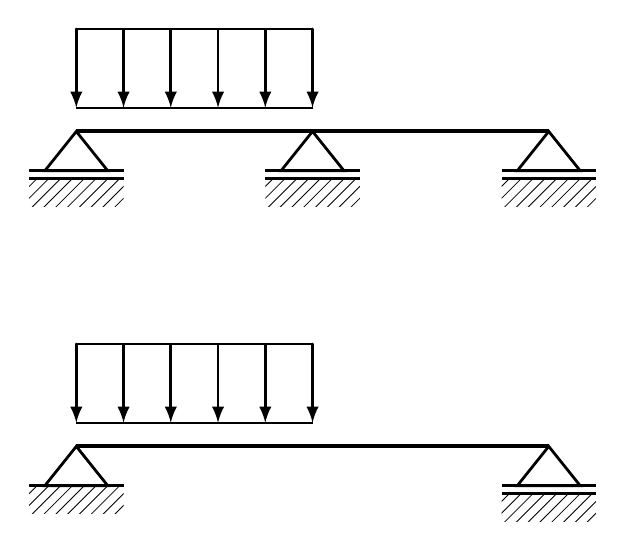
\begin{tikzpicture}
			\point{a}{0}{0};
			\point{b}{6}{0};
			\point{c}{0}{4};
			\point{d}{3}{4};
			\point{e}{6}{4};
			\point{f}{3}{0};
			\beam{2}{a}{b};
			\beam{2}{c}{e};
			\support{1}{a};
			\support{2}{b};
			\support{2}{c};
			\support{2}{d};
			\support{2}{e};
			\lineload{1}{a}{f};
			\lineload{1}{c}{d};
		\end{tikzpicture}
		\end{center}
		\end{figure}
			\textbf{Solution:}
			\begin{itemize}
				\item With no redundant support, we have an exact match for this beam in Appendix C, which gives $v_{max} = 	\US{0.029}{in} $
				\item We can use superposition again for the case with redundant reinforcement, but we treat the extra middle support as a point load such that the deflections at the center are equal, thus $\frac{5wL^4}{768EI}=\frac{PL^3}{48EI}$ which gives $P = \frac{5wL}{16} = 	\US{18.75}{lb} $
				\item We will only use equations for $0 < x < L/2$ since that is where we expect the maximum deflection to occur and we find a maximum deflection at $x = 	\US{17.01}{in} $ of $v_{max} = 	\US{0.0025}{in} $, which reduces our maximum deflection by approximately a factor of 10.
			\end{itemize}

\end{enumerate}
\end{document}
